\section{Spiral Model Demodulation}

\begin{figure}
    \centering
    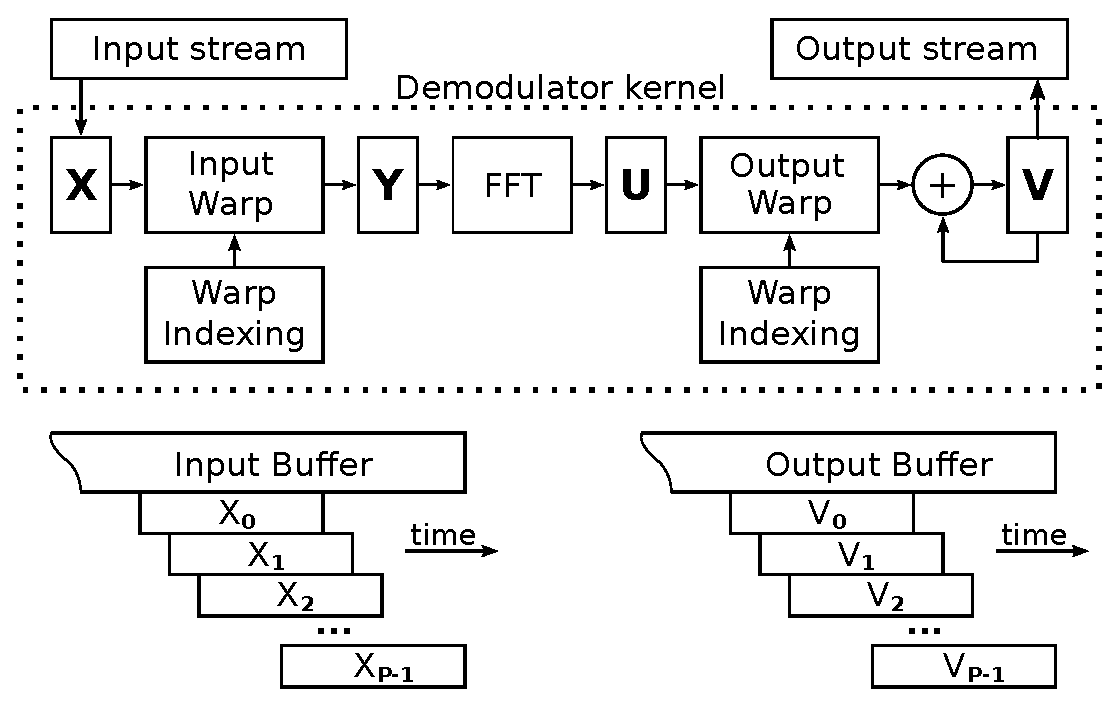
\includegraphics[width=0.95\linewidth]{../source/demod_e}
    \caption[Quantum to Relative Time Demodulation]{Demodulation data flow}
    \label{fig:demod}
\end{figure}

The mathematics of signal conversion, besides FFT, is mainly College Algebra.
The algorithm can be coded by a typical programmer or engineer with the help
from some math tricks and perhaps working around the bugs in my thinking.

%%%%%%%%%%%%%%%%%%%%%%%%%%%%%%%%%%%%%%%%%%%%%%%%%%%%%%%%%%%%%%%%%%%%%%%%%%%%%%%%
\subsection{Reference Chirp}

The most important part of a software ecosystem is its test code.
The test code for QTDSP generates a reference chirp.
That chirp is the basis for the demodulation algorithm.

Let R be a scaled version of $\omega$.
Let N be the size of the Fourier Transform, which is an exact power of two.
Typically, it's between 256 and 16384. 
Stepping $n$ from 0 to N-1,

\begin{equation}  \label{eq:tc}
f(n) = f_0 \cdot exp\left(\frac{nR}{N}\right)
\end{equation}

Computing many sequential points of transcendental functions tends to be slow.
It's better to come with a fast algorithm. With some luck, it will also illuminate   
the problem of fast signal demodulation.

Stepwise exponential growth or decay can be handled by a multiply operation.
Let $b$ be the step size for the multiplier.
Setting $e^R = (1 + b)^N$,
\begin{equation}
b = e^{R/N} - 1
\end{equation}

For each iteration:
\begin{equation}
f_{n+1} = f_n \cdot (1 + b)
\end{equation}

Since $R/N \ll 1$, the first term or two of the Maclaurin series expansion of the
exponent function is enough for a good approximation.
So, $b$ is very close to $R/N$.

%%%%%%%%%%%%%%%%%%%%%%%%%%%%%%%%%%%%%%%%%%%%%%%%%%%%%%%%%%%%%%%%%%%%%%%%%%%%%%%%
\subsection{Input Warping}

The downsampling process of Fig.~\ref{fig:demod} translates the sample pitch of
$\vec{X}$ to the sample pitch of $\vec{Y}$ using an exponential sweep.
In the industry, this is known as exponential time-warping.
The input time warp re-samples input data such that a reference chirp would get
translated to a constant-period sinusoid.

An exponential chirp sweeps from $f_0$ to $f_1$ in a time $t$.
M points of $\vec{X}$ get mapped onto N points of $\vec{Y}$, where $M < N$.
Re-sampling is done on N points (of $\vec{Y}$) at a time where the respective indices of
$\vec{X}$ and $\vec{Y}$ are $\delta$ and $i$.
$\vec{X}$ is swept from $\mathbf{X}_0$ to $\mathbf{X}_M$
or $\mathbf{X}_M$ to $\mathbf{X}_0$.

Let $\lambda$ be the sample pitch of $\vec{X}$.
It will increase or decrease exponentially and should have a maximum value of 1.

This causes a chirp of matching R to be re-sampled to the upper frequency
(either $f_0$ or $f_1$ depending on the sign of R).
Given output index i, input sample index $\delta(i)$ is the accumulated sum of
$pitch(i)$ where $pitch$ decreases exponentially from 1.0
or increases exponentially toward 1.0.
In the latter case, the initial $pitch$ can either be determined from a dummy
run of the resampling algorithm or analytically.
It's $e^{M \cdot R/N}$. 
M is derived from a geometric progression in Eq. \ref{eq:M_N0}.

\begin{equation}  \label{eq:M_N0}
N = \sum_{k=1}^{M} e^{|R| \cdot (k-1)/N} = \frac{1 - e^{|R| \cdot M/N}}{1 - e^{|R|/N}}
\end{equation}

\begin{equation}  \label{eq:M_N}
M = \frac{N}{|R|} \cdot\ ln\left( 1 - N(1-e^{|R|/N}) \right)
\end{equation}

An analytical expression of the re-sampling function ($i$ to $\delta$)
was over my head, but it's easily expressed as an algorithm.
Interpolating from a fractional $\vec{X}$ index in this example (WarpIn listing)
is done by cubic interpolation using a Catmull-Rom spline.
Given four points $y_0, y_1, y_2, y_3$, a cubic polynomial describes the curve
passing through all four points whose slope matches up between adjacent segments.
With $x$ ranging from 0 to 1 indexing the point on $[y_1, y_2]$.

\begin{equation}  \label{eq:cubic}
f = a_0 \cdot x^3 + a_1 \cdot x^2 + a_2 \cdot x + a_3
\end{equation}

\begin{lstlisting}[float,floatplacement=H]
float WarpIn(
  float* out,        // output stream
  float* in,         // input stream
  int length,        // points in output stream
  double delta,      // starting input index, 0 to 1
  double pitch,      // exponential input sample pitch
  double b,          // exp rate of change of pitch
  double amplitude,  // starting amplitude
  double fcomp)      // decay rate of amplitude
{
  float y0 = *in++;
  float y1 = *in++;
  float y2 = *in++;
  float y3 = *in++;
  // coefficients for first y1-y2 segment of the curve
  float a0 = -0.5 * y0 + 1.5 * y1 - 1.5 * y2 + 0.5 * y3;
  float a1 = y0 - 2.5 * y1 + 2.0 * y2 - 0.5 * y3;
  float a2 = -0.5 * y0 + 0.5 * y2;
  float a3 = y1;
  for (int i = 0; i < length; i++) {
    float x = delta; // between 0 and 1 on y1-y2 path
    float sum = x * (x * (x * a0 + a1) + a2) + a3;
    *out++ = sum * amplitude; // deemphasize low end
    delta += pitch;
    if (delta >= 1.0) {
      delta -= 1.0;
      pitch += pitch * b;
      amplitude += amplitude * fcomp;
      y0 = y1;       // stepped into the next segment
      y1 = y2;
      y2 = y3;
      y3 = *in++;
      a0 = -0.5 * y0 + 1.5 * y1 - 1.5 * y2 + 0.5 * y3;
      a1 = y0 - 2.5 * y1 + 2.0 * y2 - 0.5 * y3;
      a2 = -0.5 * y0 + 0.5 * y2;
      a3 = y1;
    }
  }
  return pitch;
}
\end{lstlisting}

Regardless of the sign of $R$, the input warp shifts the corresponding chirp
to the lesser of $f_0$ and $f_1$. Let $\gamma$ be the highest frequency component in the
time-warped input:

\begin{equation} \label{eq:gamma}
\gamma = \frac{N}{2} \cdot \frac{1}{1 + |R|}
\end{equation}

Note: The effect of S on $\gamma$ hasn't been tested yet.

Input interpolation produces noise artifacts, as you would expect.
They get spread broadly across the spectrum above the region of interest.
Figure \ref{fig:inwarpspec} shows the output power spectrum (10 dB/div) of
the warp function. The test chirp decays in frequency exponentially from
$0.45 F_S$ with $R=-2$.
A 4096-point Fast Fourier Transform omits the window function so you can
see the distribution of noise artifacts to the right of the peak.

\begin{figure}
  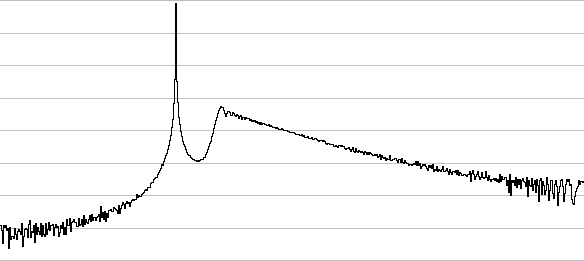
\includegraphics[width=\linewidth]{../source/inwarpspec.png}
  \caption{$f_1$ peak of warped exponential chirp, with artifacts.}
  \label{fig:inwarpspec}
\end{figure}

That's a great relief because it removes any need for much more
compute-intensive resampling algorithms. Warping may be kept simple and fast.


%%%%%%%%%%%%%%%%%%%%%%%%%%%%%%%%%%%%%%%%%%%%%%%%%%%%%%%%%%%%%%%%%%%%%%%%%%%%%%%
\subsection{FFT}

After $\vec{X}$ is time-warped into $\vec{Y}$, $\vec{Y}$ is processed by a
Fast Fourier Transform and converted to data set $\vec{U}$ containing N/2
frequency bins. Not all of them are used.
Outputs above $\gamma$ (Eq. \ref{eq:gamma}) are ignored.

$\vec{Y}$ and $\vec{U}$ may share the
same physical memory if the FFT is performed in place.
The output of the FFT is converted to the square of the magnitude for use in
RMS averaging, so square root is not needed.

A window function $w(n)$ is applied to Y before performing the FFT.
Hann and Nuttall windows are both good functions, with a tradeoff between
peak spreading and dynamic range.
Eq. \ref{eq:hann} is the Hann window function.

\begin{equation} \label{eq:hann}
w(n) = \frac{1}{2}\left(1 - cos\left( \frac{2\pi n}{N-1} \right)\right)
\end{equation}

Given N input points, output indices up to $\frac {0.5 \cdot N}{1 + |R|}$
are used for further processing.


%%%%%%%%%%%%%%%%%%%%%%%%%%%%%%%%%%%%%%%%%%%%%%%%%%%%%%%%%%%%%%%%%%%%%%%%%%%%%%%%
\subsection{Output Warping}

$\vec{U}$ is upsampled to form time-domain signal $\vec{V}$.
Let $\epsilon$ and $j$ be the respective indices of $\vec{U}$ and $\vec{V}$.
The maximum usable value of $\epsilon$ is $\gamma$ (Eq. \ref{eq:gamma}).
Integer index $j$ steps one at a time while $\epsilon$ decays exponentially.

Warp indexing uses the relation:
\begin{equation}
\epsilon = \gamma e^{\omega(t - \tau)}
\end{equation}

Time $t$ (scaled to match the output stream's sample rate) sweeps from $\tau$
in the opposite direction of R's sign,
causing the exponent to start at 1 and decay downward.

$j$ sweeps downward from $\gamma(N/2-1)$.
Index $\epsilon(j)$ is independent of R.

\begin{equation}  \label{eq:eps_j}
\epsilon(j) = \gamma e^{-kj/N}
\end{equation}

The desired difference between $\epsilon(0)$ and $\epsilon(1)$ in
Eq. \ref{eq:eps_j} is $1$. $\epsilon(0) = \gamma$
and $\epsilon(1) = \gamma e^{-k/N}$,
which gives a $k$ of about $-2|R|$:

\begin{equation}  \label{eq:k}
k = N \cdot ln \left(1 - 2 \cdot \frac{|R| + 1}{N} \right)
\end{equation}

The exponential decay of $\epsilon$ can be handled by repeated multiplication,
one per $\vec{U}_\epsilon$ fetch.
The exponential sweep needs a small correction factor to have a base of exactly
$e$.
%\frac{N}{2} \cdot (1 - e^{-k})
Setting $e^{k} = (1 + \zeta)^{N}$,
\begin{equation}
\zeta = e^{k/N} - 1
\end{equation}

Sample C code for the output warp:

\begin{lstlisting}[float,floatplacement=H]
static void WarpOut(
  float* out,               // output stream (V)
  float* in,                // input stream (mag^2)
  int length,
  double gamma,             // max epsilon index
  double zeta,              // rate of change of gamma
  float fcomp)              // decay rate of amplitude
{
  int idx0 = (int)gamma;
  in = &in[idx0 + 1];       // -> first point
  double epsilon = gamma;
  float amplitude = 1.0f;
  float y1 = *in--;
  float y0 = *in--;
  float a0 = y1 - y0;
  float a1 = y0;
  for (int i = 0; i < length; i++) {
    float idx1 = idx0;
    float x = gamma - idx0; // between 0 and 1 on y0-y1
    float sum = x * a0 + a1;
    *out++ = sum * amplitude; // deemphasize low end
    amplitude += amplitude * fcomp;
    gamma += gamma * zeta;  // epsilon exponentially decays
    idx0 = (int)gamma;
    if (idx0 != idx1) {
      y1 = y0;              // stepped into the next segment
      y0 = *in--;
      a0 = y1 - y0;
      a1 = y0;
    }
  }
}
\end{lstlisting}


%%%%%%%%%%%%%%%%%%%%%%%%%%%%%%%%%%%%%%%%%%%%%%%%%%%%%%%%%%%%%%%%%%%%%%%%%%%%%%%%
\subsection{Correlation}

Let $H_X$ be the integer number of new X samples per conversion.

Let $H_V$ be the real number of output samples per conversion.
Combining Eq. \ref{eq:gamma} and Eq. \ref{eq:k} gives:

\begin{equation}  \label{eq:hv}
H_V = H_X \cdot \frac{R}{N} \cdot \frac{R}{|R| + 1}
          \cdot \frac{-1}{ln(1 - \frac{2|R|}{N})}
\end{equation}

Since $\epsilon$ is always positive, the upchirp case of $R>0$ needs to have its
j index mirrored by using $\vec{U}_{v-j}$, where v is the maximum j such as (15/32)N.
The warp output is added to $\vec{V}$ memory as described below, indexed from the
top or bottom of the active region of V.

Warped $\vec{U}$ is added to output buffer $\vec{V}$ by summation,
staggered in time (by $H_V$ samples) for each processing block.
When the downsampler's R value matches the chirp rate of an incoming chirp,
multiple peaks in the warped FFT output correlate in the output stream to
produce a corresponding output pulse in the $\vec{V}$ stream.
A more complex signal such as overlapping and/or modulated chirps will produce
pulse trains and/or modulation envelopes in the $\vec{V}$ stream.

$\vec{U}$ is in logarithmic format so that summing a bunch of them is basically 
repeated multiplication.
It's cheaper than actual multiplication and less subject to overflow.
Multiplying (or summing logs) of linearized spectra is a form of cross-correlation.
The sum can be normalized with a scale that's the inverse of the V oversampling:

\begin{equation}
scale = -H_X \cdot \frac{R^2}{ln(1 - \frac{2|R|}{N})}
\end{equation} % (n / 2) / (1 + fabs(r))

\begin{figure}
    \centering
    \includegraphics[width=0.99\linewidth]{../source/wbuf_e}
    \caption[$\vec{V}$ correlation]{Correlation of $\vec{V}$}
    \label{fig:wbuf}
\end{figure}

Fig.~\ref{fig:wbuf} shows the output correlator, another view of buffer $\vec{V}$.
The output stream flows from left to right,
being initialized to 0 outside the accumulation region.
After $U_\epsilon$ is added to $\vec{V}$, the $V_0$ index moves $H_V$ points
to the left, leaving $H_V$ newly minted output points.

Elements of $\vec{V}$ are accumulated squares of magnitudes.
An attempt was made to accumulate vectors,
with the idea that the phase rotations might sync up,
but it didn't work in simulation.
So, angle data from the FFT is discarded.

\section{Parabolic Model Demodulation}

The parabolic time model is simpler than the spiral model.
There's no correlator. A spectrum analyzer is also easier to build.

%%%%%%%%%%%%%%%%%%%%%%%%%%%%%%%%%%%%%%%%%%%%%%%%%%%%%%%%%%%%%%%%%%%%%%%%%%%%%%%%
\subsection{Reference Chirp}

The parabolic chirp has a frequency that starts at $F_0$ and ends at 0.
Its frequency forms half of a parabola when $N$ points are plotted.

%%%%%%%%%%%%%%%%%%%%%%%%%%%%%%%%%%%%%%%%%%%%%%%%%%%%%%%%%%%%%%%%%%%%%%%%%%%%%%%%
\subsection{Input Warping}

The downsampling process of Fig.~\ref{fig:demod} translates the sample pitch of
$\vec{X}$ to the sample pitch of $\vec{Y}$ using a parabolic sweep.
The input time warp re-samples input data such that a reference chirp would get
translated to a constant-period sinusoid.

M points of $\vec{X}$ get mapped onto N points of $\vec{Y}$, where $M = 0.468N$.
The chirp's $F_0$ gets down-sampled by a factor of 3.53 to match $F_1$,
the frequency at $X[M]$.
As with the spiral model, such down-sampling is well-behaved.
Upsampling $F_1$ to $F_0$ would be more difficult and need anti-aliasing filtering.

Rather than showing a mathematical derivation,
a code listing of the time warping tells all. 
Cubic interpolation via Catmull-Rom spline is again used.

\begin{lstlisting}[float,floatplacement=H]
void ParabolicWarp(
  float* out,       // output stream
  float* in,        // input stream
  int n,            // points in output stream
  float pitch)      // exponential input sample pitch
{
  float y0, a0, a1, a2, a3;
  float y1 = *in++;
  float y2 = *in++;
  float y3 = *in++;
  float x = 0;      // between 0 and 1 on y1-y2 path
  float dp = n;     // dharma point is at right edge
  float dp0 = sqrtf(pitch) * dp;
  pitch = 1.0;
  for (int i = 0; i < n; i++) {
    x += pitch;
    if (x >= 1.0) { // stepped into the next segment
      x -= 1.0;
      float s = dp0 / dp;
      pitch = s * s;
      dp--;
      y0 = y1;
      y1 = y2;
      y2 = y3;
      y3 = *in++;
      // coefficients for y1-y2 segment of the cubic curve
      a0 = -0.5f * y0 + 1.5f * y1 - 1.5f * y2 + 0.5f * y3;
      a1 = y0 - 2.5f * y1 + 2.0f * y2 - 0.5f * y3;
      a2 = -0.5f * y0 + 0.5f * y2;
      a3 = y1;
    }
    *out++ = x * (x * (x * a0 + a1) + a2) + a3;
  }
}
\end{lstlisting}

After $\vec{X}$ is time-warped into $\vec{Y}$, $\vec{Y}$ is processed by a
Fast Fourier Transform and converted to magnitude data $\vec{U}$ containing N/2
frequency bins. Not all of them are used.
Outputs above $F_S / 7$ are ignored.

Given N input points, output indices up to $F_S / 7$
are used for further processing.

%%%%%%%%%%%%%%%%%%%%%%%%%%%%%%%%%%%%%%%%%%%%%%%%%%%%%%%%%%%%%%%%%%%%%%%%%%%%%%%%
\subsection{Spectral Display for Parabolic Time}

The FFT output can be used to form a column of heat-mapped pixels on a display.
Each subsequent conversion forms another column.
$H_X$ samples are appended to $\vec{X}$ for each new conversion.
A GPU would typically run hundreds of warps and FFTs in parallel to produce a
2D image as a single processing block.

Since there is no correlation step, the parabolic chirp is smeared across the
output image.
Figure \ref{fig:p4kbw3} illustrates the image produced by a test waveform.
$F_0$ is $F_S/2$.
At $F_0$, the smear is thinnest.
The high frequency components of the smear are the most pronounced at $F_0$.
A 2D FFT can be used to help pick out the location of the chirp.

\begin{figure}
  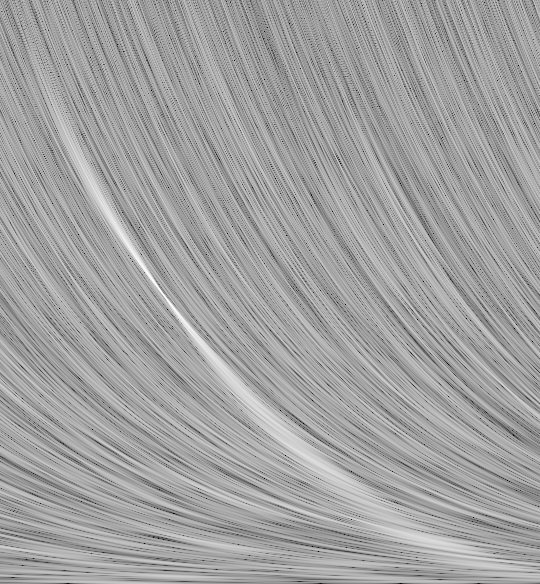
\includegraphics[width=0.8\linewidth]{../source/p4kbw3.jpg}
  \caption{Parabolic chirp 3dB below noise.}
  \label{fig:p4kbw3}
\end{figure}

